%%%%%%%%%%%%%%%%%%%%%%%%%%%%%%%%%%%%%%%%%%%%
%%%%% Template made by: @KelvynTownley %%%%%
%%%%%%%%%%%%%%%%%%%%%%%%%%%%%%%%%%%%%%%%%%%%
\documentclass[letterpaper, 11pt]{article}	% You can change 'article' for 'assignment' or antoher document class
\usepackage[letterpaper, margin=2.1cm]{geometry}
% You can change the value of 'margin' for another one.
% You can also set the margin of the top, bottom, left or right side individually using the following keywords:
% 'top=<here the value><System of Units (cm, in, em, pt)>'
% 'left=<here the value><System of Units (cm, in, em, pt)>'
% 'right=<here the value><System of Units (cm, in, em, pt)>'
% 'bottom=<here the value><System of Units (cm, in, em, pt)>'
\usepackage[utf8]{inputenc}	% Not recommended to change it
\usepackage[english]{babel}	% This adapts some formats such as titles and dates depending on the language and region; for example, sections in Spanish would say "sección" and in English would say "section" or dates in Spanish would say "noviembre 202X" and in English "November 202X".
\usepackage{amsmath, amssymb, amsthm, wasysym}	% Packages required for some mathematical notations.
\usepackage[skins]{tcolorbox}	% Package required to create fancy boxes.
\usepackage{color, xcolor}	% Packages required to use colors in the document.
\usepackage{graphicx, tikz}	% Packages required to create graphics and use images.
	\usetikzlibrary{calc, decorations.pathmorphing}	% Required to do beauty decorations.
\usepackage{fancyhdr}	% Package required to set creative headers and footers.
\usepackage{microtype}	% To solve some almost insignificant problems.
\usepackage{float}	% Package required to move any figure.

% The following change the font family to Sans Serif
\usepackage{charter}
\renewcommand{\familydefault}{\sfdefault}

% The following commands define new colors as variables. (HTML means Hexadecimal)
% In the first '{}' you can change the name color for anyone dou you want.
% In the last '{}' you can change the hexadecimal code of the color, you can search in internet for someone do you want.
\definecolor{neonPurple}{HTML}{B983FF}
\definecolor{neonBlue}{HTML}{94B3FD}
\definecolor{neonCyan}{HTML}{94DAFF}


\begin{document}

\pagestyle{empty}	% You can delete it so that the document is automatically numbered.
\begin{tikzpicture}[remember picture, overlay]
	% I recommend that you only change the fill colors in the following block.
	% I do not recommend that you change other parameters unless you know what you are doing.
	\fill[fill=neonPurple] ($(current page.north west) - (0,6)$) -- (current page.north east) -- ($(current page.north west) - (0,0)$) -- ($(current page.north west) - (0,6)$);
	\fill[fill=neonBlue] ($(current page.north east) + (0,-5)$) -- (current page.north) -- ($(current page.north east) + (0,0)$) -- ($(current page.north east) + (0,-5)$);
	
	% You can change the text that is in the last '{}' of 'subject' and 'name'.
	\node[text=white, font=\Huge\bfseries, anchor=north west] (subject) at ($(current page.north west) + (2,-1.3)$) {Discrete Mathematics};	% You can change "Discrete Mathematics"
	\node[text=white, font=\Large\bfseries, anchor=north west] (studentName) at ($(current page.north west) + (2,-2.5)$) {Kelvyn Townley};	% You can change "Kelvyn Townley"
	\node[text=white, font=\large\bfseries, anchor=north east] (date) at ($(current page.north east) - (1,1.5)$) {\today};	% I do not recommend that you change the date "\today" but also is possible.
\end{tikzpicture}

\vspace*{3cm} % DO NOT DELETE THIS LINE.
% In the following line, you can change the text color "neonPurple" and also you can change the instructions "Research... applications".
\noindent {\Large \textcolor{neonPurple}{\textbf{Instructions}: Research about \textit{The Pigeonhole Principle} and develop examples of its applications.}}\\[5mm]

% The following line is a subtitle with my personal set, you can use it or discard it. 
\noindent \textcolor{neonBlue}{\textbf{\large About The Pigeonhole Principle}}\\

% From here you must write on your own. What follows are only test notes.
\noindent The Pigeonhole principle says:
\begin{tcolorbox}[colback=white, colframe=neonBlue, leftrule=3mm, sharp corners]
	If n pigeonholes are occupied by n+1 pigeons, at least one pigeonhole is occupied by more than one pigeon.
\end{tcolorbox}

\noindent In fact, from a mathematical perspective, let $p$ be the pigeons and $h$ the pigeonholes, then at least one pigeonhole contains at least $\frac{p}{h}$ pigeons.\\

\noindent \textcolor{neonBlue}{\textbf{\large Examples with applications}}

\begin{enumerate}
	\item If $m$ is an odd positive integer, then prove that there exists a positive integer $n$ such that $m$ divides $2^n-1$.\\[5mm]
		Let $m$ be an odd positive integer, we consider the finite sequence of powers of 2:
		\begin{equation*}
			2^1,2^2,...,2^m.  
		\end{equation*}
		Since $m$ is odd, it does not divide to any of the above powers. So the possible remainders of $2^i\div m$ (with $1\leq i \leq m$) are:
		\begin{equation*}
			1,\ 2,\ ...,\ m-1 
		\end{equation*}
		Since there are $m-1$ possible remainders (pigeonholes) and $m$ powers of 2 (pigeons), it follows that there exist at least two positive integers $p$ and $q$ (say $p < q \leq m$) such that $2^p$ and $2^q$ have the same remainders in the division by $m$. Thus, it turns out that $m$ divides $2^q-2^p$. Let us note that
		\begin{equation*}
			2^q-2^p=2^p(2^{q-p}-1) 
		\end{equation*}
		Since $p$ and $q$ are positive integers, with $p < q$, then $q-p$ is a positive integer (say $n$) and since $m$ does not divide $2^p$, then $m$ divides $2^{n}-1$.
		
		$\therefore$ There is a positive integer $n$ such that $m$ divides $2^n-1$.\\[3cm]
	\item Show that if any eight positive integers are chosen, two of them will have the same remainder when divided by 7.\\[5mm]	
	The remainders that result from dividing any positive integer by $7$ are: $\{0, 1, 2, 3, 4, 5, 6\}$; that is, seven possibilities, which can be considered as the pigeonholes, under the analogy of the pigeonhole principle, as shown:
		\begin{center}
			\fbox{\textcolor{gray}{$0$}} \fbox{\textcolor{gray}{$1$}} \fbox{\textcolor{gray}{$2$}} \fbox{\textcolor{gray}{$3$}} \fbox{\textcolor{gray}{$4$}} \fbox{\textcolor{gray}{$5$}} \fbox{\textcolor{gray}{$6$}}
		\end{center}
		
		Then we take 8 integers (inhabitants) that when arranged in the houses, by principle of the pigeonhole, at least in one pigeonhole, there will be more than one inhabitant, as shown:
		\begin{center}
			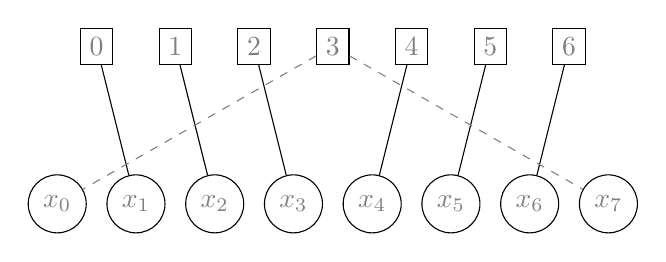
\begin{tikzpicture}
				%%% PALOMARES
				\node[rectangle, text=gray, draw=black] (0) at (.5,0) {$0$};
				\node[rectangle, text=gray, draw=black] (1) at (1.5,0) {$1$};
				\node[rectangle, text=gray, draw=black] (2) at (2.5,0) {$2$};
				\node[rectangle, text=gray, draw=black] (3) at (3.5,0) {$3$};
				\node[rectangle, text=gray, draw=black] (4) at (4.5,0) {$4$};
				\node[rectangle, text=gray, draw=black] (5) at (5.5,0) {$5$};
				\node[rectangle, text=gray, draw=black] (6) at (6.5,0) {$6$};
				
				%%% PALOMAS
				\node[circle, text=gray, draw=black] (x0) at (0,-2) {$x_0$};
				\node[circle, text=gray, draw=black] (x1) at (1,-2) {$x_1$};
				\node[circle, text=gray, draw=black] (x2) at (2,-2) {$x_2$};
				\node[circle, text=gray, draw=black] (x3) at (3,-2) {$x_3$};
				\node[circle, text=gray, draw=black] (x4) at (4,-2) {$x_4$};
				\node[circle, text=gray, draw=black] (x5) at (5,-2) {$x_5$};
				\node[circle, text=gray, draw=black] (x6) at (6,-2) {$x_6$};
				\node[circle, text=gray, draw=black] (x7) at (7,-2) {$x_7$};
				
				%%% CONEXIONES
				\draw (0) -- (x1);
				\draw (1) -- (x2);
				\draw (2) -- (x3);
				\draw[dashed, gray] (3) -- (x0);
				\draw (4) -- (x4);
				\draw (5) -- (x5);
				\draw (6) -- (x6);
				\draw[dashed, gray] (3) -- (x7);
			\end{tikzpicture}
		\end{center}
\end{enumerate}

\end{document}